\documentclass[10pt,a4paper]{article}

% Language setting
% Replace `english' with e.g. `spanish' to change the document language
\usepackage[utf8]{inputenc}
\usepackage[latin1]{inputenc}

% Set page size and margins
% Replace `letterpaper' with`a4paper' for UK/EU standard size
\usepackage[letterpaper,top=2cm,bottom=2cm,left=3cm,right=3cm,marginparwidth=1.75cm]{geometry}

% Useful packages
\usepackage{amsmath}
\usepackage{graphicx}
\usepackage[colorlinks=true, allcolors=blue]{hyperref}
\usepackage{float}
\usepackage{listings}
\usepackage{color}
\usepackage{listingsutf8}
\usepackage{enumitem}
\usepackage[demo]{graphicx}
\usepackage{subfig}

\definecolor{dkgreen}{rgb}{0,0.6,0}
\definecolor{gray}{rgb}{0.5,0.5,0.5}
\definecolor{mauve}{rgb}{0.58,0,0.82}

\lstset{frame=tb,
  language=Java,
  aboveskip=3mm,
  belowskip=3mm,
  showstringspaces=false,
  columns=flexible,
  basicstyle={\small\ttfamily},
  numbers=none,
  numberstyle=\tiny\color{gray},
  keywordstyle=\color{blue},
  commentstyle=\color{dkgreen},
  stringstyle=\color{mauve},
  breaklines=true,
  breakatwhitespace=true,
  tabsize=3,
  literate=%
    {ã}{{\'a}}1
    {á}{{\'a}}1
    {é}{{\'e}}1
}

\title{Documentação de atividades para o Grupo 5 \\ Processamento de Iamgens Digitais \\ Professor Leandro Alves Neves}
\author{Anderson Garrido Scaioni \\ Andréia Salmazo Bertasso \\ Johny W. Alves (johnywalves@gmai.com)}

\begin{document}
\maketitle

\section{Uso pacotes e criação da biblioteca}

\begin{flushleft}
Foram instaladas os pacotes do Python Package Index (PyPI), um repositório de software para a linguagem de programação Python, fazendo uso do comando
\end{flushleft}

\begin{lstlisting}[language=Bash]
pip install pillow matplotlib scikit-learn
\end{lstlisting}

\begin{flushleft}
Para facilitar a apresentação dos resultados posteriores e algumas rotinas foram usadas algumas funções reutilizadas
\end{flushleft}

\lstinputlisting[language=Python]{library.py}

\section{Criação e Rotulagem de Imagens - Exercício 6}

\subsection{Enunciado}

Escreva um programa para reproduzir as imagens apresentadas no slide 41. Considere que as imagens têm dimensões: 256x256 com 256 níveis de profundidade. Em seguida, o programa deve ser capaz de apresentar a taxa de amostragem e a profundidade de cada imagem.

\subsection{Código Fonte}

\lstinputlisting[language=Python]{01_generate_images.py}

\subsection{Explicação}

\begin{flushleft}
O programa para geração de imagens foi criado na linguagem Python e utiliza o pacote “Pillow”, foi definida a função {\ttfamily create\textunderscore images(name, quantization)} que cria a imagem com os parâmetros name (nome da imagem) e quantization (quantificação dos cinzas), nessa função {\ttfamily img = Image.new('P', (256, 256))} a imagem criada é de 8 bits de profundidade com tamanho 256x256 pixels, após a geração da imagem ela é salva em disco na pasta images com a extensão bmp conforme o seguinte código  {\ttfamily  img.save('./images/' + name + '.bmp')}.
\end{flushleft}

\begin{flushleft}
A função é executada 5 vezes, para gerar assim as imagens a.bmp, b.bmp, c.bmp, d.bmp e e.bmp na pasta images.  
\end{flushleft}

\begin{figure}[H]
    \centering
    \subfloat[\centering a.bmp]{{
\includegraphics[width=2cm]{a.jpg}}}%
    \qquad
    \subfloat[\centering b.bmp]{{
\includegraphics[width=2cm]{b.jpg}}}%
    \qquad
    \subfloat[\centering c.bmp]{{
\includegraphics[width=2cm]{c.jpg}}}%
    \qquad
    \subfloat[\centering d.bmp]{{
\includegraphics[width=2cm]{d.jpg}}}%
    \qquad
    \subfloat[\centering e.bmp]{{
\includegraphics[width=2cm]{e.jpg}}}%
\end{figure}

\section{Criação e Rotulagem de Imagens - Exercício 11}

\subsection{Enunciado}

\begin{flushleft}
Considere as imagens produzidas no Exercício 6 e implemente um programa para realizar a rotulagem de componentes conexos (cluster/aglomerado). A rotulagem deve ser realizada por meio do “Hoshen–Kopelman algorithm”. O programa deve fornecer o total de componentes conexos e os rótulos atribuídos em cada região da imagem dada como entrada. Use vizinhança-8 como critério. Por fim, considerando a imagem (e) após a rotulagem, o programa deve apresentar as distâncias (D\textsubscript{e}, D\textsubscript{4} e D\textsubscript{8}) entre os centros de dois componentes conexos (definidos (sorteados) aleatoriamente).
\end{flushleft}

\subsection{Código Fonte}

\lstinputlisting[language=Python]{02_clustering_images.py}

\subsection{Explicação}

\begin{flushleft}
A implementação do algortimo para clursterização tem como base o algoritmo de rotulagem "Hoshen-Kopelman", adaptado para utilizar vizinhaça 8 e agrupar pela quantização de cinza, a linguagem de programação é Python juntamente com o pacote "Pillow".
\end{flushleft}

\begin{flushleft}
Definido o número de linhas e colunas (256x256) vindo das imagens e um vetor com as possíveis cores a rotulagem.
\end{flushleft}

\begin{flushleft}
Três funções para calcular a distância foram implementadas:
\end{flushleft}

\begin{itemize}
    \item {\ttfamily distance\textunderscore euclidean(first, second)};
    \item {\ttfamily distance\textunderscore four(first, second)};
    \item {\ttfamily distance\textunderscore eight(first, second)}.
\end{itemize}

\begin{flushleft}
A função {\ttfamily cluster\textunderscore image(name)} realiza a rotulagem através de cores e quando executada utiliza as funções:
\end{flushleft}

\begin{itemize}
   \item {\ttfamily find(labels, x)};
   \item {\ttfamily union(labels, x, y)}.
 \end{itemize}

\begin{flushleft}
A imagem clursterizada é salva na pasta "images" com o nome da imagem original adicionado de "\textunderscore clustered.bmp", após a imagem ser salva é exibido nome da imagem original, quantidade de grupos e rótulos dos grupos. 
\end{flushleft}

\begin{flushleft}
Se a imagem a ser clursterizada for a imagem "e.bmp" é calculada as distância euclidiana, distância quatro (\textit{city-block}) e distância oito (\textit{chessboard}) de dois aglomerados conexos, selecionados aleatoriamente e verificados pela função {\ttfamily is\textunderscore connected(first, second)}
\end{flushleft}

 \begin{flushleft}
A função {\ttfamily cluster\textunderscore image} é executada 5 vezes uma para cada imagem gerada no exercício anterior.
\end{flushleft}

\lstinputlisting[language=Bash]{02_clustering_images.txt}

\section{Ruído - Exercício 4}

\subsection{Enunciado}

Dada a imagem (e) com e sem a presença de ruído gaussiano (exercício 3), compare-as por meio das métricas  \textit{erro máximo}, \textit{erro médio absoluto}, \textit{erro médio quadrático}, \textit{raiz do erro médio quadrático}, \textit{erro médio quadrático normalizado} e \textit{coeficiente de Jaccard} para identificar os níveis de similaridades existentes.

\begin{enumerate}[label=\roman*.]
    \item Observando os valores obtidos, é possível definir algum comportamento padrão entre as métricas a partir dos ruídos aplicados em cada imagem?
    \item Neste cenário, qual métrica permite evidenciar melhor a degradação da imagem em razão da presença de ruído? Justifique sua resposta.
\end{enumerate}

\subsection{Código Fonte}

\lstinputlisting[language=Python]{03_noise_gaussian.py}

\subsection{Saída}

\lstinputlisting[language=Python]{03_noise_gaussian.txt}

\subsection{Conclusão}

\begin{enumerate}[label=\roman*.]
\item Observando os valores obtidos, é possível definir um padrão de picos inversamente proporcional ao histograma da imagem original de forma que o coeficiente de Jacard indica similidade entre as duas imagens, mostra bem a deterioração do conteúdo original

\begin{figure}[H]
    \centering
    \subfloat[\centering Imagem original]{{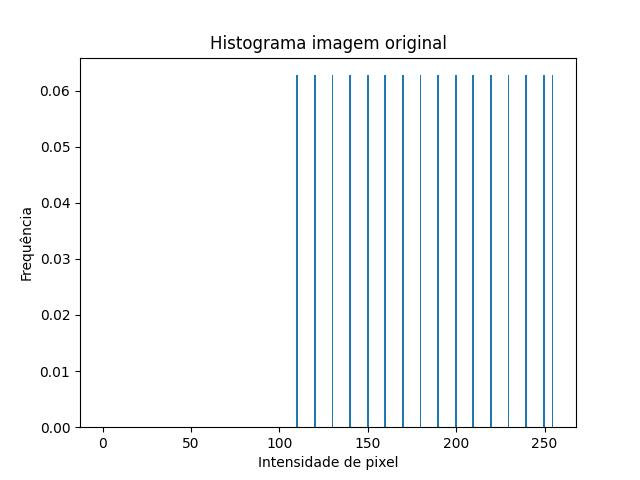
\includegraphics[width=4.5cm]{e_histogram.jpg}}}%
    \qquad
    \subfloat[\centering Ruído gaussiano]{{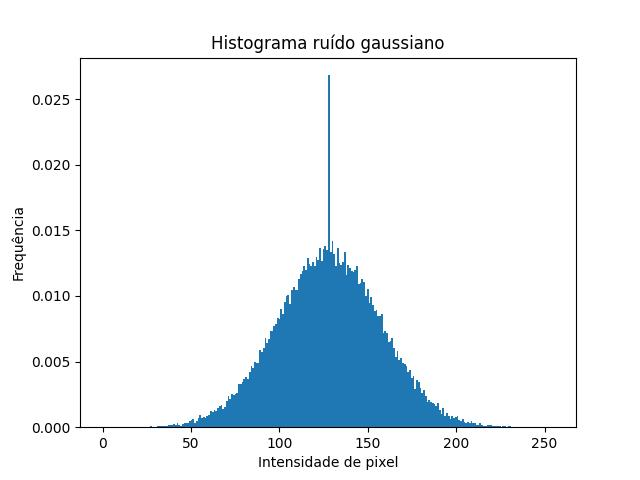
\includegraphics[width=4.5cm]{noise_histogram.jpg}}}%
    \qquad
    \subfloat[\centering Imagem ruidosa]{{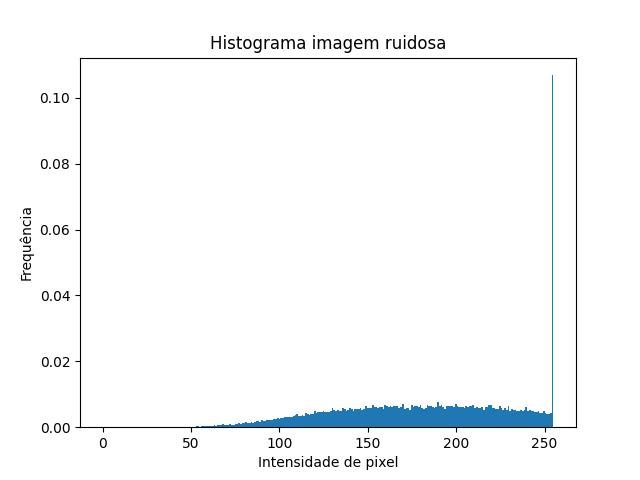
\includegraphics[width=4.5cm]{e_noised_histogram.jpg}}}%
\end{figure}

\item O erro médio quadrático com resultado 94.27720642089844 para o desvio padrão de 30 por possuir uma variância maior sobre os outros valores que permite evidenciar melhor a degradação da imagem em razão da presença de ruído, evidenciado pela figura e\textunderscore noise\textunderscore gaussian.bmp apresentado abaixo

\begin{figure}[H]
    \centering
    
\includegraphics[scale=0.9]{e_noise_gaussian.jpg}
    \caption{Figura e\textunderscore noise\textunderscore gaussian.bmp}
    \label{fig:enoisegausian}
\end{figure}

\end{enumerate}


\section{Ruído - Exercício 5}

\subsection{Enunciado}

Descreva cada etapa para ilustrar o processo de aplicação de ruídos em uma imagem A (5x5), com níveis de cinza definidos aleatoriamente. Para tanto, determine os parâmetros
iniciais para produzir uma imagem B (representativa do ruído em questão) e, em seguida, apresente: 

\begin{enumerate}[label=\alph*.]
   \item o resultado da função p(z);
   \item a imagem B representativa do ruído;
   \item o histograma de B para mostrar a característica do ruído;
   \item a matriz A após ser degrada por B;
   \item o histograma do resultado obtido em (d).
\end{enumerate}

 Esses experimentos devem ser realizados com os ruídos gaussiano e poisson (shot noise) ou salt-and-pepper noise.

\subsection{Código Fonte}

\lstinputlisting[language=Python]{04_noise_gaussian_poisson.py}

\subsection{Saída}

\lstinputlisting[language=Python]{04_noise_gaussian_poisson.txt}

\begin{figure}[H]
    \centering
    \subfloat[\centering Função p(z) do ruído de Gaussiano]{{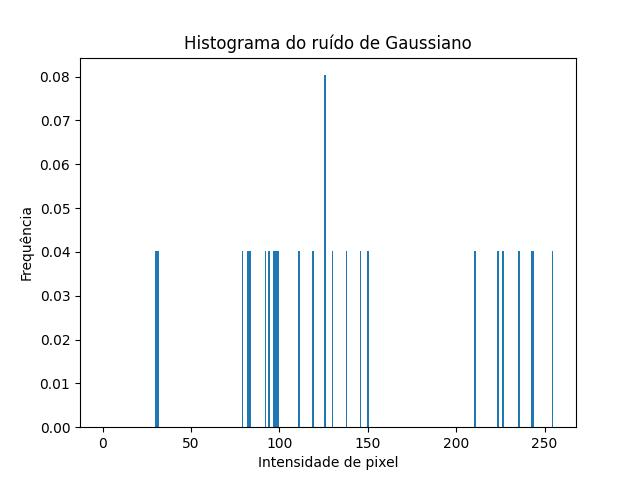
\includegraphics[width=6cm]{pz_gauss_degraded.jpg}}}%
    \qquad
    \subfloat[\centering Histograma do ruído de Gaussiano]{{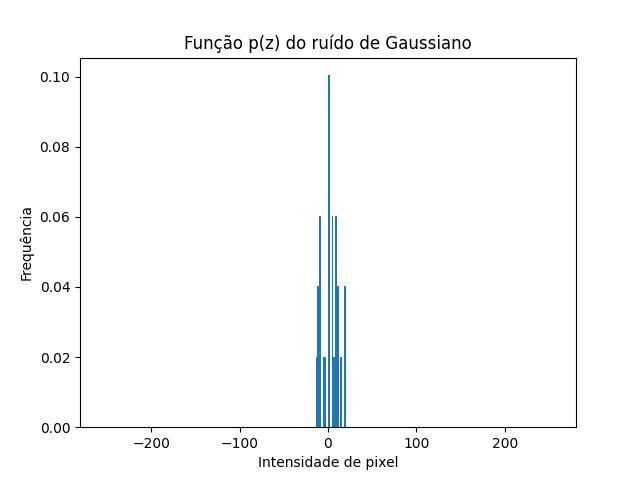
\includegraphics[width=6cm]{pz_gauss_noise.jpg}}}%
    \qquad
    \centering
    \subfloat[\centering Função p(z) do ruído Poisson]{{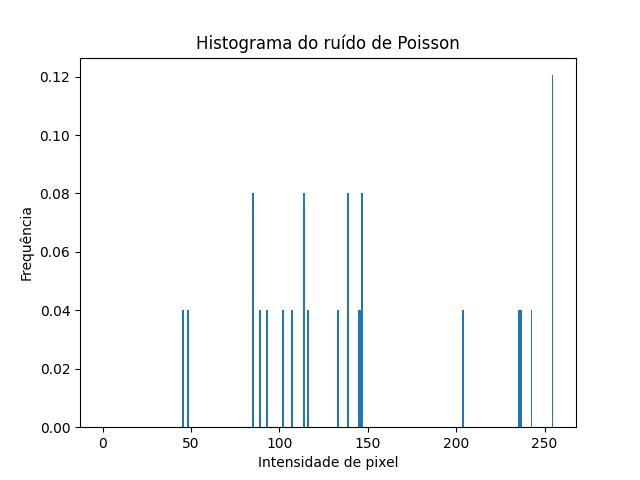
\includegraphics[width=6cm]{pz_poisson_degraded.jpg}}}%
    \qquad
    \subfloat[\centering Histograma do ruído de Poison]{{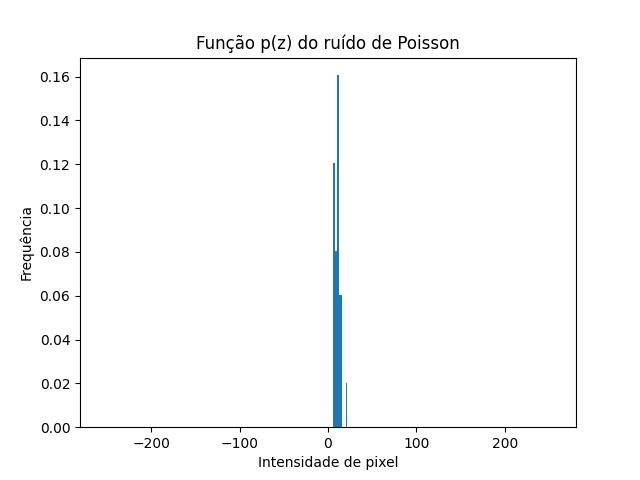
\includegraphics[width=6cm]{pz_poisson_noise.jpg}}}%
    \qquad
\end{figure}

\end{document}